         \chapter{The atom}\fancyfoot[LO,RE]{Chemistry: Matter and Materials}
\label{chap:atom}
%     \setcounter{figure}{1}
%     \setcounter{subfigure}{1}
    \label{ea1c9e59656f96ee804546971cf6dee6}
    \label{m38756*cid1}
            \section{Introduction}
            \nopagebreak
%            \label{m38756} $ \hspace{-5pt}\begin{array}{cccccccccccc}   
\includegraphics[width=0.75cm]{col11305.imgs/summary_video.png} &   \end{array} $ \hspace{2 pt}\raisebox{-5 pt}{} {(section shortcode: P10019 )} \par   
      \par \label{m38756*id254141}We have now looked at many examples of the types of matter and materials that exist around us and we have investigated some of the ways that materials are classified. But what is it that makes up these materials? And what makes one material different from another? In order to understand this, we need to take a closer look at the building blocks of matter - the \textbf{atom}. Atoms are the basis of all the structures and organisms in the universe. The planets, sun, grass, trees, air we breathe and people are all made up of different combinations of atoms.\par 
\chapterstartvideo{VPrkk}
%     \setcounter{subfigure}{0}
% 	\begin{figure}[H] % horizontal\label{m38756*the-atom-1}
%     \textnormal{Veritasium video on the atom - 1} \nopagebreak
%   \label{m38756*yt-media10}\label{m38756*yt-video10}
%             \raisebox{-5 pt}{ 
\includegraphics[width=0.5cm]{col11305.imgs/summary_www.png}} { (Video:  P10020 )}
%  \end{figure} 
    \label{m38756*eip-613}
            \begin{project}{Library assignment: Models of the atom}
            \nopagebreak
            \label{m38756*eip-3}

Our current understanding of the atom came about over a long period of time, with many different people playing a role. Conduct some research into the development of at least five different ideas of the atom and the people who contributed to it.\\ \newline
\begin{minipage}{.6\textwidth}
Some suggested people to look at are: JJ Thomson, Ernest Rutherford, Marie Curie, JC Maxwell, Max Planck, Albert Einstein, Niels Bohr, Lucretius, LV de Broglie, CJ Davisson, LH Germer, Chadwick, Werner Heisenberg, Max Born, Erwin Schrodinger, John Dalton, Empedocles, Leucippus, Democritus, Epicurus, Zosimos, Maria the Jewess, Geber, Rhazes, Robert Boyle, Henry Cavendish, A Lavoisier and H Becquerel. You do not need to find information on all these people, but try to find information about as many of them as possible.
\label{m38756*id7342}Make a list of five key contributions to a model of the atom and then make a timeline of this information. (You can use an online tool such as Dipity (http://www.dipity.com/) to make a timeline.) Try to get a feel for how it all eventually fit together into the modern understanding of the atom. 
\end{minipage}
\begin{minipage}{.4\textwidth}
 \begin{center}
\textbf{A timeline of atomic theory}
  \includegraphics[height=1.2\textwidth]{photos/timeline_atom.png}
 \end{center}

\end{minipage}

\end{project}

            \section{Models of the atom}
            \nopagebreak
      \label{m38756*id254164}It is important to realise that a lot of what we know about the structure of atoms has been developed over a long period of time. This is often how scientific knowledge develops, with one person building on the ideas of someone else. We are going to look at how our modern understanding of the atom has evolved over time.\\ 
\mindsetvid{The origins of atomic theory}{VPakv}
      \label{m38756*id254508}The idea of atoms was invented by two Greek philosophers, Democritus and Leucippus in the fifth century BC. The Greek word $\alpha \tau \text{o}\mu \text{o}\nu$ (atom) means \textbf{indivisible} because they believed that atoms could not be broken into smaller pieces.\\ 
      \label{m38756*id254540}Nowadays, we know that atoms are made up of a \textbf{positively charged nucleus} in the centre
surrounded by \textbf{negatively charged electrons}. However, in the past, before the structure of the atom was properly understood, scientists came up with lots of different \textbf{models} or \textbf{pictures} to describe what atoms look like. 

\Definition{ Model } { A model is a representation of a system in the real world. Models help us to understand systems and their properties.} 
 For example, an \textsl{atomic model} represents what the structure of an atom \textsl{could} look like, based on what we know about how atoms behave. It is not necessarily a true picture of the exact structure of an atom. \\
Models are often simplified. The small toy cars that you may have played with as a child are models. They give you a good idea of what a real car looks like, but they are much smaller and much simpler. A model cannot always be absolutely accurate and it is important that we realise this, so that we do not build up an incorrect idea about something.
\subsection*{Dalton's model of the atom}
\begin{minipage}{.5\textwidth}
John Dalton proposed that all matter is composed of very small things which he called atoms. This was not a completely new concept as the ancient Greeks (notably Democritus) had proposed that all matter is composed of small, indivisible (cannot be divided) objects. When Dalton proposed his model electrons and the nucleus were unknown.  
\end{minipage}
\begin{minipage}{.5\textwidth}
%    \setcounter{subfigure}{0}
	\begin{figure}[H] % horizontal\label{m38756*uid2}
    \begin{center}
\scalebox{.8}{
\begin{pspicture}(-3,-3)(3,3)
%\psgrid[gridcolor=lightgray]
\pscircle(0,0){1}
\end{pspicture}
}
% \begin{minipage}{.8\textwidth}
\caption{The atom according to Dalton}
% \end{minipage}
% \label{fig:atom:dalton}
\end{center}
 \end{figure}
\end{minipage}

      \label{m38756*uid1}
            \subsection*{Thomson's model of the atom}
            \nopagebreak
\begin{minipage}{.5\textwidth}
        \label{m38756*id254616}After the electron was discovered by J.J. Thomson in 1897, people realised that atoms were made up of even smaller particles than they had previously thought. However, the atomic nucleus had not been discovered yet and so the ``plum pudding model'' was put forward in 1904. In this model, the atom is made up of negative electrons that float in a ``soup'' of positive charge, much like plums in a pudding or raisins in a fruit cake (figure~\ref{fig:atom:plumpudding}). In 1906, Thomson was awarded the Nobel Prize for his work in this field. However, even with the Plum Pudding Model, there was still no understanding of how these electrons in the atom were arranged.\par 
\end{minipage}
\begin{minipage}{.5\textwidth}
%     \setcounter{subfigure}{0}
	\begin{figure}[H] % horizontal\label{m38756*uid2}
    \begin{center}
\scalebox{.7}{
\begin{pspicture}(-3,-3)(3,3)
%\psgrid[gridcolor=lightgray]
\psellipse(0,0)(2.5,2.5)
\psline[linewidth=0.3cm](0,2)(0,-2)
\psline[linewidth=0.3cm](-2,0)(2,0)
\psellipse(-1.5,1.5)(0.25,0.25)
\rput(-1.5,1.5){\textbf{-}}
\psellipse(-1,1)(0.25,0.25)
\rput(-1,1){\textbf{-}}
\psellipse(-1.5,-1)(0.25,0.25)
\rput(-1.5,-1){\textbf{-}}
\psellipse(-1,-1.5)(0.25,0.25)
\rput(-1,-1.5){\textbf{-}}
\psellipse(1,1.5)(0.25,0.25)
\rput(1,1.5){\textbf{-}}
\psellipse(1.5,-1.5)(0.25,0.25)
\rput(1.5,-1.5){\textbf{-}}
\psellipse(1,0.5)(0.25,0.25)
\rput(1,0.5){\textbf{-}}
\psellipse(1,-1)(0.25,0.25)
\rput(1,-1){\textbf{-}}
\psline(1.2,1.6)(3,1.6)
\rput(4,1.6){\textbf{electrons}}
\psline(2,-1)(3,-1)
\rput(3.8,-1){\textbf{'soup' of}}
\rput(4.3,-1.5){\textbf{positive charge}}
\end{pspicture}
}
\begin{minipage}{.8\textwidth}
\caption{The atom according \\ to the Plum Pudding model}
\end{minipage}
\label{fig:atom:plumpudding}
\end{center}
 \end{figure}    
\end{minipage}  
\par
\IFact{Two other models proposed for the atom were the cubic model and the Saturnian model. In the cubic model, the electrons were imagined to lie at the corners of a cube. In the Saturnian model, the electrons were imagined to orbit a very big, heavy nucleus.}
        \label{m38756*id254642}The discovery of \textbf{radiation} was the next step along the path to building an accurate picture of atomic structure. In the early twentieth century, Marie and Pierre Curie, discovered that some elements (the \textsl{radioactive} elements) emit particles, which are able to pass through matter in a similar way to X-rays (read more about this in Grade 11). It was Ernest Rutherford who, in 1911, used this discovery to revise the model of the atom.\par 
      \label{m38756*eip-956}

      \label{m38756*uid3}
            \subsection*{Rutherford's model of the atom}
            \nopagebreak
\begin{minipage}{.5\textwidth}
            \label{m38756*id254751}Rutherford carried out some experiments which led to a change in ideas around the atom. His new model described the atom as a tiny, dense, positively charged core called a nucleus surrounded by lighter, negatively charged electrons. Another way of thinking about this model was that the atom was seen to be like a mini solar system where the electrons orbit the nucleus like planets orbiting around the sun. A simplified picture of this is shown alongside. This model is sometimes known as the planetary model of the atom.\\
\end{minipage}
\begin{minipage}{.5\textwidth}
%     \setcounter{subfigure}{0}
	\begin{figure}[H] % horizontal\label{m38756*uid5}
    \begin{center}
\scalebox{.8}{
\begin{pspicture}(-2.2,-2.4)(2.2,2.4)
\SpecialCoor
%\psgrid%[gridcolor=lightgray]
\def\water{\psset{unit=0.2}\rput{150}{\pscircle[fillcolor=white,fillstyle=solid](0,0){2}
\psarc[fillcolor=white,fillstyle=solid](-1.5,1){1.5}{30}{260}
\psarc[fillcolor=white,fillstyle=solid](1.5,1){1.5}{280}{150}
\rput(-1.5,1){\pscurve(1.5;30)(-1;142.5)(1.5;260)}
\rput(1.5,1){\pscurve(1.5;150)(-1;37.5)(1.5;280)}}}

\def\atom{\rput(0,0){\water}\rput{180}(0.25,0.25){\water}\rput{45}(0.25,0.25){\water}\rput{225}(0.25,0.25){\water}}

\rput(0,0){\atom}
\psellipse[linecolor=lightgray,linewidth=3pt](0,0)(1.5,2.2)
\rput{120}{\psellipse[linecolor=lightgray,linewidth=3pt](0,0)(1.5,2.2)}
\rput{240}{\psellipse[linecolor=lightgray,linewidth=3pt](0,0)(1.5,2.2)}

\psdots[dotsize=5pt](1,1.6)(-1,-1.6)\uput[ur](1,1.6){electron orbiting the nucleus}
\rput{120}{\psdots[dotsize=5pt](1,1.6)(-1,-1.6)}
\rput{240}{\psdots[dotsize=5pt](1,1.6)(-1,-1.6)}
\uput[r](2.4,0){nucleus}
\psline{<-}(1,0)(2.4,0)
\end{pspicture}
}
\caption{Rutherford's model of the atom}
\end{center}
\label{rutherfordmodel}
 \end{figure} 
\end{minipage}      
      \label{m38756*uid6}
            \subsection*{Bohr's model of the atom}
            \nopagebreak
\begin{minipage}{.5\textwidth}
        \label{m38756*id254784}There were, however, some problems with Rutherford's model: for example it could not explain the very interesting
observation that atoms only emit light at certain wavelengths or frequencies. Niels Bohr solved this problem by proposing that the electrons could only orbit the nucleus in certain special orbits at different energy levels around the nucleus.\\
\end{minipage}
\begin{minipage}{.5\textwidth}
   \setcounter{subfigure}{0}
	\begin{figure}[H] % horizontal\label{m38756*uid2}
    \begin{center}
\scalebox{.5}{
\begin{pspicture}(-6,-6)(6,6)
%\psgrid[gridcolor=lightgray]
\pscircle[fillstyle=solid,fillcolor=gray](0,0){0.1}
\pscircle[linecolor=darkgray,linewidth=0.1](0,0){1}
\pscircle[linecolor=darkgray,linewidth=0.1](0,0){2}
\pscircle[linecolor=darkgray,linewidth=0.1](0,0){3}
\psline[linewidth=0.05]{<-}(0.1,0)(4,0)
\uput[r](4,0){\Large{nucleus}}
\psline[linewidth=0.05]{<-}(1.8,1)(4,1)
\uput[r](4,1){\Large{electron orbit}}
\end{pspicture}
}
\begin{minipage}{.8\textwidth}
\caption{Bohr's model of the atom}
\end{minipage}
\label{fig:atom:dalton}
\end{center}
 \end{figure}
\end{minipage}

\label{m38756*notfhsst!!!underscore!!!id119}
\subsection*{James Chadwick}
Rutherford predicted (in 1920) that another kind of particle must be present in the nucleus along with the proton. He predicted this because if there were only positively charged protons in the nucleus, then it should break into bits because of the repulsive forces between the like-charged protons! To make sure that the atom stays electrically neutral, this particle would have to be neutral itself. In 1932 James Chadwick discovered the neutron and measured its mass.
\label{m38756*eip-279}
            \subsection*{Other models of the atom}
            \nopagebreak
            \label{m38756*eip-993}
Although the most commonly used model of the atom is the Bohr model, scientists are still developing new and improved theories on what the atom looks like. One of the most important contributions to atomic theory (the field of science that looks at atoms) was the development of quantum theory. Schrodinger, Heisenberg, Born and many others have had a role in developing quantum theory.  
\par \label{m38756*eip-179}
            \begin{exercises}{Models of the atom}
            \nopagebreak \vspace{-1cm}
            \label{m38756*eip-786}Match the information in column A, with the key discoverer in column B.
          \begin{table}[H]
        \begin{center}
      \label{m38756*eip-551}
      \begin{tabular}{|l|l|}\hline
        \textbf{Column A} &
        \textbf{Column B} \\ \hline
        \textbf{1.} Discovery of electrons and the plum pudding model &
        \textbf{A.} Niels Bohr \\ \hline
        \textbf{2.} Arrangement of electrons &
        \textbf{B.} Marie and Pierre Curie  \\ \hline
        \textbf{3.} Atoms as the smallest building block of matter &
        \textbf{C.} Ancient Greeks and Dalton \\ \hline
        \textbf{4.} Discovery of the nucleus &
        \textbf{D.} JJ Thomson \\ \hline
        \textbf{5.} Discovery of radiation &
        \textbf{E.} Rutherford \\ \hline
    \end{tabular}
      \end{center}
\end{table}
\practiceinfo
 \begin{tabular}[h]{cccccc}
 (1.) 000k  & \end{tabular}
\end{exercises}
            \section{Atomic mass and diameter}
            \nopagebreak
            \label{m38756*id254850}It is difficult sometimes to imagine the size of an atom, or its mass, because we cannot see an atom and also because we are not used to working with such small measurements. 
            \subsection*{How heavy is an atom?}
            \nopagebreak
        \label{m38756*id254863}It is possible to determine the mass of a single atom in kilograms. But to do this, you would need special instruments and the values you would get would be very clumsy and difficult to work with. The mass of a carbon atom, for example, is about $1,99 \times {10}^{-26}\text{ kg}$, while the mass of an atom of hydrogen is about $1,67 \times{10}^{-27}\text{ kg}$. Looking at these very small numbers makes it difficult to compare how much bigger the mass of one atom is when compared to another.\\ 
        \label{m38756*id254908}To make the situation simpler, scientists use a different unit of mass when they are describing the mass of an atom. This unit is called the \textbf{atomic mass unit} (amu). We can abbreviate (shorten) this unit to just u. Scientists use the \textbf{carbon standard} to determine amu. The carbon standard gives carbon an atomic mass of $12,0 \text{ u}$. Compared to carbon the mass of a hydrogen atom will be $1 \text{ u}$. Atomic mass units are therefore not giving us the \textsl{actual} mass of an atom, but rather its mass \textsl{relative} to the mass of one (carefully chosen) atom in the periodic table. In other words it is only a number in comparison to another number. The atomic masses of some elements are shown in table~\ref{tab:atomic mass}.

          \begin{table}[H]
        \begin{center}
      \label{m38756*uid8}
    \noindent
      \begin{tabular}{|l|l|}\hline
\textbf{Element} & \textbf{Atomic mass (u)} \\ \hline
Carbon ($\text{C}$) & $12,0$ \\ \hline
Nitrogen ($\text{N}$) & $14,0$ \\ \hline
Bromine ($\text{Br}$) & $79,9$ \\ \hline
Magnesium ($\text{Mg}$) & $24,3$ \\ \hline
Potassium ($\text{K}$) & $39,1$ \\ \hline
Calcium ($\text{Ca}$) & $40,1$ \\ \hline
Oxygen ($\text{O}$) & $16,0$ \\ \hline
    \end{tabular}
      \end{center}
    \caption{The atomic mass number of some of the elements.}
\label{tab:atomic mass}
\end{table}
        \label{m38756*id255096}The actual value of 1 atomic mass unit is $1,67 \times {10}^{-24} \text{ g}$ or $1,67 \times {10}^{-27} \text{ kg}$. This is a very tiny mass! If we write it out it looks like this: $0,000~000~000~000~000~000~000~000~167\text{ kg}$. An atom is therefore very very small. 

            \subsection*{Rutherford's alpha-particle scattering experiment}
            \nopagebreak
            \label{m38756*id254668}Radioactive elements emit different types of particles. Some of these are positively charged alpha ($\alpha $) particles.
Rutherford wanted to find out where the positive charge in an atom is. He carried out a series of experiments where he bombarded sheets of gold foil with alpha particles (since these would be repelled by the positive nucleus). A simplified diagram of his experiment is shown in figure~\ref{fig:atom:goldfoil}.

\begin{figure}[H] % horizontal\label{m38756*uid4}
 \begin{center}
\scalebox{.8}{
\begin{pspicture}(-4,-3)(9,3)
\SpecialCoor
%\psgrid%[gridcolor=lightgray]

\def\gold{\pscircle(0,0){0.2}\psdot(0,0)}

\rput(0,0){
\psarc[linewidth=2pt](0,0){3}{270}{90}
\psframe[fillcolor=lightgray,fillstyle=solid](-0.2,-2)(0,2)
\psframe[fillcolor=white,fillstyle=solid](-4,-0.5)(-2,0.5)
\rput(-3,0.2){radioactive}
\uput[d](-3,0.2){substance}
\psline[linewidth=1.5pt]{->}(-2,0)(-0.2,0)
\uput[d](-1.1,0){$\alpha$ particles}
\psline[linestyle=dashed](-0.2,0)(-2,3)
\uput[dr](-1.8,3){C}
\psline[linestyle=dashed](-0.2,0)(-2,-3)
\uput[ur](-1.8,-3){C}

\psline[linestyle=dashed](0,0)(2,2.2)
\uput[l](2,2.2){B}
\psline[linestyle=dashed](0,0)(2,-2.2)
\uput[l](2,-2.2){B}

\psline[linestyle=dashed](0,0)(3,0)
\psline[linestyle=dashed](0,0)(3,0.2)
\uput[ul](3,0.2){A}
\psline[linestyle=dashed](0,0)(3,-0.2)
\uput[dl](3,-0.2){A}

\uput[ur](1.3,-3){Zinc Sulfide screen}}

\rput(5,0){
\psframe(0,-2)(1,2)
\multirput(0.2,-1.8)(0,0.4){10}{\gold}
\multirput(0.5,-1.6)(0,0.4){9}{\gold}
\multirput(0.8,-1.8)(0,0.4){10}{\gold}

\psline{->}(-1,1.5)(2,1.5)\uput[ul](2,1.5){A}
\psline{->}(-1,0.35)(0.5,0.35)(2,0)\uput[ul](2,0){B}
\psline{->}(-1,-1)(0.2,-1)(-1,-2)\uput[u](-1,-2){C}
\pcline[linestyle=none](-1,-2)(-1,2)
\lput*{:U}{$\alpha$ particles}
\psline(0.8,-1.4)(1.4,-1.4)
\rput[l](1.4,-1.4){nucleus of}
\uput[dr](1.4,-1.5){gold atom}

}
\rput(-3,-2.5){(a)}
\rput(5.5,-2.5){(b)}
\psline(-0.2,1.5)(-2,1.5)
\rput(-3,1.5){gold sheet}
\end{pspicture}
}
\caption{Rutherford's gold foil experiment. Figure (a) shows the path of the $\alpha$ particles after they hit the gold sheet. Figure (b) shows the arrangement of atoms in the gold sheets and the path of the $\alpha$ particles in relation to this.}
\label{fig:atom:goldfoil}
\end{center}
\end{figure}
\mindsetvid{The Rutherford model}{VPald}       
\label{m38756*id254715}Rutherford set up his experiment so that a beam of alpha particles was directed at the gold sheets. Behind the gold sheets was a screen made of zinc sulphide. This screen allowed Rutherford to see where the alpha particles were landing. Rutherford knew that the \textsl{electrons} in the gold atoms would not really affect the path of the alpha particles, because the mass of an electron is so much smaller than that of a proton. He reasoned that the positively charged \textsl{protons} would be the ones to \textsl{repel} the positively charged alpha particles and alter their path.\par 
If Thomson's model of the atom was correct then Rutherford would have observed mostly path C in figure~\ref{fig:atom:goldfoil}. (C represents alpha particles that are reflected by the positive nucleus). What he found instead was that most of the alpha particles passed through the foil undisturbed and could be detected on the screen directly behind the foil (path A). Some of the particles ended up being slightly deflected onto other parts of the screen (path B).  The fact that most particles passed straight through suggested that the positive charge was concentrated in one part of the atom only.\par 
Through this experiment he concluded that the nucleus of the atom is positively charged and situated in the middle of the atom.
\subsection*{How small is the nucleus?}
\begin{minipage}{.5\textwidth}
The nucleus of an atom is very small. We can compare an atom with a soccer stadium. If the whole atom is as big as a soccer stadium, the nucleus is only the size of a pea in the middle of the stadium! This should help you see that the atom is mainly made up of empty space. If you removed all the empty space from the atoms in your body, you would become the size of a grain of salt!
\end{minipage}
\begin{minipage}{.5\textwidth}
\begin{center}
\textbf{A stadium}\\
 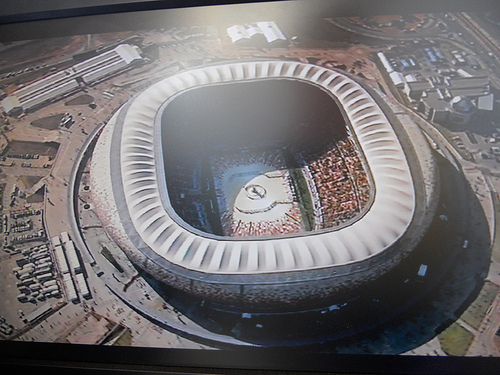
\includegraphics[width=.4\textwidth]{photos/stadiumby-shine2010-flickr.jpg}\\
\textit{Picture by Shine 2010 on Flickr.com}
\end{center}
\end{minipage}
      \label{m38756*eip-491}
            \subsection*{Relative atomic mass}
            \nopagebreak

\Definition{ Relative atomic mass } {The relative atomic mass of an element is the average mass of all the naturally occurring isotopes of that element. The units for relative atomic mass are atomic mass units.} 

The relative atomic mass of an element is the number you will find on the periodic table.  
         \section{Structure of the atom}
    \nopagebreak
%            \label{m38745} $ \hspace{-5pt}\begin{array}{cccccccccccc}   
\includegraphics[width=0.75cm]{col11305.imgs/summary_fullmarks.png} &   \end{array} $ \hspace{2 pt}\raisebox{-5 pt}{} {(section shortcode: P10021 )} \par 
    \label{m38745*cid4}
            \nopagebreak
      \label{m38745*id255206}As a result of the work done by previous scientists on atomic models, scientists now have a good idea of what an atom looks like. This knowledge is important because it helps us to understand why materials have different properties and why some materials bond with others. Let us now take a closer look at the microscopic structure of the atom (what the atom looks like inside). \\ 
\mindsetvid{the nucleus}{VPaln}
      \label{m38745*id255216}So far, we have discussed that atoms are made up of a positively charged \textbf{nucleus} surrounded by
one or more negatively charged \textbf{electrons}. These electrons orbit the nucleus.\\ 
      \label{m38745*eip-577}Before we look at some useful concepts we first need to understand what electrons, protons and neutrons are. \label{m38745*uid10}
            \subsection*{The Electron}
            \nopagebreak
The electron is a very tiny particle. It has a mass of $9,11 \times {10}^{-31} \text{ kg}$. The electron carries one unit of negative electric charge (i.e.\@{} $-1,6 \times 10^{-19} \text{ C}$).
      \label{m38745*uid11}
            \subsection*{The Nucleus}
            \nopagebreak
Unlike the electron, the nucleus \textbf{can} be broken up into smaller building blocks called \textbf{protons} and \textbf{neutrons}. Together, the protons and neutrons are called \textbf{nucleons}.
        \label{m38745*uid12}
            \subsubsection*{The Proton}
\IFact{Scientists believe that the electron can be treated as a \textbf{point particle} or \textbf{elementary particle} meaning that it cannot be broken down into anything smaller.} The electron carries one unit of \textbf{negative} electric charge (i.e.\@{} $-1,6 \times {10}^{-19} \text{ C}$, C is Coulombs).
           \nopagebreak
          \label{m38745*id255338}Each proton carries one unit of \textbf{positive} electric charge (i.e.\@{} $+1,6 \times {10}^{-19} \text{ C}$).
Since we know that atoms are \textbf{electrically neutral}, i.e.\@{} do not carry any extra charge, then the number of protons in an atom has to be the same as the number of electrons to balance out the positive and negative charge to zero. The total positive charge of a nucleus is equal to the number of protons in the nucleus. The proton is much heavier than the electron ($10~000$ times heavier!) and has a mass of $1,6726 \times {10}^{-27} \text{ kg}$. When we talk about the atomic mass of an atom, we are mostly referring to the combined mass of the protons and neutrons, i.e.\@{} the nucleons.
        \label{m38745*uid13}
            \subsubsection*{The Neutron}
            \nopagebreak
          \label{m38745*id254468}The neutron is electrically neutral i.e.\@{} it carries no charge at all.
Like the proton, it is much heavier than the electron and its mass is $1,6749 \times {10}^{-27} \text{ kg}$ (slightly heavier than the proton).\par 
\label{m38745*notfhsst!!!underscore!!!id214}
    % \textbf{m38745*uid14}\par
          \begin{table}[H]
    % \begin{table}[H]
    % \\ '' '0'
        \begin{center}
      \label{m38745*uid14}
    \noindent
      \begin{tabular}{|l|l|l|l|}\hline
         &
                    \textbf{proton}
                   &
                    \textbf{neutron}
                   &
                    \textbf{electron} \\ \hline
                    \textbf{Mass (kg)}
                   &
        $1,6726 \times {10}^{-27}$ &
        $1,6749 \times {10}^{-27}$ &
        $9,11 \times {10}^{-31}$ \\ \hline
                    \textbf{Units of charge}
                   &
        $+1$ &
        $0$ &
        $-1$ \\ \hline
                    \textbf{Charge (C)}
                   &
        $1,6 \times {10}^{-19}$ &
        $0$ &
        $-1,6 \times {10}^{-19}$ \\ \hline
    \end{tabular}
      \end{center}
    \caption{Summary of the particles inside the atom}
\end{table}
    \par
    \label{m38745*cid5}
            \subsection*{Atomic number and atomic mass number}
            \nopagebreak
      \label{m38745*id255805}The chemical properties of an element are determined by the charge of its nucleus, i.e.\@{} by the \textbf{number of protons}. This number is called the \textbf{atomic number} and is denoted by the letter \textbf{Z}.

\Definition{ Atomic number (Z) } { The number of protons in an atom  } 
      
\label{m38745*eip-164}You can find the atomic number on the periodic table (see periodic table at front of book). The atomic number is an integer and ranges from $1$ to about $118$.\par 
\label{m38745*id255845}The mass of an atom depends on how many nucleons its nucleus contains.
The number of nucleons, i.e.\@{} the total number of protons \textbf{plus} neutrons,
is called the \textbf{atomic mass number} and is denoted by the letter \textbf{A}.\\
\IFact{Currently element 118 is the highest atomic number for an element. Elements of high atomic numbers (from about 93 to 118) do not exist for long as they break apart within seconds of being formed. Scientists believe that after element 118 there may be an ``island of stability'' in which elements of higher atomic number occur that do not break apart within seconds.}
\Definition{Atomic mass number (A) } {The number of protons and neutrons in the nucleus of an atom  } 

The atomic number (Z) and the mass number (A) are indicated using a standard notation, for example carbon will look like this: $_{6}^{12}\text{C}$

      \label{m38753*id255886}Standard notation shows the chemical symbol, the atomic mass number
and the atomic number of an element as follows:\par 
      \label{m38753*id255890}
    \setcounter{subfigure}{0}
	\begin{figure}[H] % horizontal\label{m38753*id255893}
    \begin{center}
\scalebox{1} % Change this value to rescale the drawing.
{
\begin{pspicture}(0,-1.2192708)(8.541979,1.2192708)
\usefont{T1}{ptm}{m}{n}
\rput(4.2689586,-0.0765625){\Large $^A_Z$}
\usefont{T1}{ptm}{m}{n}
\rput(4.6527085,-0.0965625){\LARGE $X$}
\psline[linewidth=0.02cm,arrowsize=0.113cm 2.5,arrowlength=1.4,arrowinset=0.0]{->}(3.203646,0.8034375)(4.1636457,0.1034375)
\psline[linewidth=0.02cm,arrowsize=0.113cm 2.5,arrowlength=1.4,arrowinset=0.0]{->}(3.203646,-0.8965625)(4.083646,-0.4165625)
\psline[linewidth=0.02cm,arrowsize=0.113cm 2.5,arrowlength=1.4,arrowinset=0.0]{<-}(4.923646,-0.1165625)(5.8036456,-0.1165625)
\usefont{T1}{ptm}{m}{n}
\rput(7.163802,-0.1065625){\psframebox[linewidth=0.02]{chemical symbol}}
\usefont{T1}{ptm}{m}{n}
\rput(1.5463021,0.9134375){\psframebox[linewidth=0.02]{number of nucleons}}
\usefont{T1}{ptm}{m}{n}
\rput(1.6763021,-0.8665625){\psframebox[linewidth=0.02]{number of protons}}
\end{pspicture} 
}
\end{center}
 \end{figure}       
 

\IFact{A nuclide is a distinct kind of atom or nucleus characterised by the number of protons and neutrons in the atom. To be absolutely correct, when we represent atoms like we do here, then we should call them nuclides.}
      
\label{m38753*id255900}For example, the iron nucleus which has $26$ protons and $30$ neutrons, is denoted as:\par 
      \label{m38753*id255904}\nopagebreak\noindent{}      
    \begin{equation*}
    _{26}^{56}\text{Fe} 
      \end{equation*}
      \label{m38753*id255929}where the atomic number is $Z=26$ and the mass number $A=56$. The number of neutrons is simply the difference $N=A-Z=30$.\par 

\Tip{Do not confuse the notation we have used here with the way this information appears on the periodic table. On the periodic table, the atomic number usually appears in the top left-hand corner of the block or immediately above the element's symbol. The number below the element's symbol is its \textbf{relative atomic mass}. This is not exactly the same as the atomic mass number. This will be explained in "Isotopes". The example of iron is shown below.
      \label{m38745*id256180}
    \setcounter{subfigure}{0}
	\begin{figure}[H] % horizontal\label{m38745*id256183}
    \begin{center}
\begin{pspicture}(-2,-2)(2,2)
\psframe(-1,-1)(1,1)
\rput(0,0){\textbf{Fe}}
\rput(-0.7,0.7){26}
\rput(0,-0.7){55.85}
\end{pspicture}
\end{center}
 \end{figure}
}

\label{m38745*eip-950} 
      \noindent 
\label{m38745*eip-222}For a neutral atom the number of electrons is the same as the number of protons, since the charge on the atom must balance. But what happens if an atom gains or loses electrons? Does it mean that the atom will still be part of the same element? A change in the number of electrons of an atom does not change the type of atom that it is. However, the charge of the atom will change. The \textsl{neutrality} of the atom has changed. If electrons are \textsl{added}, then the atom will become more \textsl{negative}. If electrons are \textsl{taken away} then the atom will become more \textsl{positive}. The atom that is formed in either of these two cases is called an \textbf{ion}. An ion is a charged atom. For example: a neutral sodium atom can lose one electron to become a positively charged sodium atom ($\text{Na}^{+}$). A neutral chlorine atom can gain one electron to become a negatively charged chlorine ion ($\text{Cl}^{-}$). Another example is $\text{Li}^{+}$ which has lost one electron and now has only $2$ electrons, instead of $3$. Or consider $\text{F}^{-}$ which has gained one electron and now has $10$ electrons instead of $9$.   
\begin{wex}
{%title
Standard notation
}
{%question
Use standard notation to represent sodium and give the number of protons, neutrons and electrons in the element.
}
{%Answer
\westep{Give the element symbol} $\text{Na}$
\westep{Find the number of protons} Sodium has 11 protons, so we have: ${}_{11}\text{Na}$
\westep{Find the number of electrons} Sodium is neutral, so it has the same number of electrons as protons. The number of electrons is 11.
\westep{Find A} From the periodic table we see that $A=23$.
\westep{Work out the number of neutrons} We know $A$ and $Z$ so we can find $N$: $N = A - Z = 23 - 11 = 12$.
\westep{Write the answer} In standard notation sodium is given by: $_{11}^{23}\text{Na}$. The number of protons is 11, the number of neutrons is 12 and the number of electrons is 11.
}    
\end{wex}
    

\begin{exercises}{The structure of the atom} \noindent \nopagebreak \vspace{-1cm}
%Question 1
      \label{m38745*id256225}\begin{enumerate}[noitemsep, label=\textbf{\arabic*}. ] 
            \label{m38745*uid15}\item Explain the meaning of each of the following terms:
\label{m38745*id256240}\begin{enumerate}[noitemsep, label=\textbf{\alph*}. ] 
            \label{m38745*uid16}\item nucleus
\label{m38745*uid17}\item electron
\label{m38745*uid18}\item atomic mass
\end{enumerate}
%Question 2
                \label{m38745*uid19}\item Complete the following table:
    % \textbf{m38745*id256298}\par
\begin{center} 
\begin{tabular}{|p{1.4cm}|p{1.4cm}|p{1.4cm}|p{2cm}|p{2cm}|p{2cm}|}\hline
\textbf{Element} & \textbf{Atomic mass units} & \textbf{Atomic number} & \textbf{Number of protons} & \textbf{Number of electrons} & \textbf{Number of neutrons}\\\hline
Mg & 24 & 12 & & & \\\hline
O & & & 8 & & \\\hline
 & & 17 & & & \\\hline
Ni & & & & 28 & \\\hline
 & 40 & & & & 20 \\\hline
Zn & & & & & \\\hline
 & & & & & 0 \\\hline
C & 12 & & & 6 & \\\hline 
$\text{Al}^{3+}$ &  & 13 & & &  \\ \hline
$\text{O}^{2-}$ & & & & 18 &  \\ \hline
\end{tabular}
\end{center}
    \par
%Question 3
          \label{m38745*uid20}\item Use standard notation to represent the following elements:
\label{m38745*id256772}\begin{enumerate}[noitemsep, label=\textbf{\alph*}. ] 
            \label{m38745*uid21}\item potassium
\label{m38745*uid22}\item copper
\label{m38745*uid23}\item chlorine
\end{enumerate}
%Question 4
                \label{m38745*uid24}\item 
For the element $_{17}^{35}\text{Cl}$, give the number of...
\label{m38745*id256843}\begin{enumerate}[noitemsep, label=\textbf{\alph*}. ] 
            \label{m38745*uid25}\item protons
\label{m38745*uid26}\item neutrons
\label{m38745*uid27}\item electrons
\end{enumerate}
... in the atom.\newline
%Question 5
\label{m38745*uid28}\item Which of the following atoms has 7 electrons?
\label{m38745*id256898}\begin{enumerate}[noitemsep, label=\textbf{\alph*}. ] 
            \label{m38745*uid29}\item $_{2}^{5}\text{He}$
\label{m38745*uid30}\item $_{6}^{13}\text{C}$
\label{m38745*uid31}\item $_{3}^{7}\text{Li}$
\label{m38745*uid32}\item $_{7}^{15}\text{N}$
\end{enumerate}
%Question 6
                \label{m38745*uid33}\item 
In each of the following cases, give the number or the element symbol represented by X.
\label{m38745*id257023}\begin{enumerate}[noitemsep, label=\textbf{\alph*}. ] 
            \label{m38745*uid34}\item $_{18}^{40}\text{X}$
\label{m38745*uid35}\item $_{20}^{x}\text{Ca}$
\label{m38745*uid36}\item $_{x}^{31}\text{P}$
\end{enumerate}
%Question 7
                \label{m38745*uid37}\item 
Complete the following table:
    % \textbf{m38745*id257121}\par
          \begin{table}[H]
    % \begin{table}[H]
    % \\ 'id2886554' '1'
        \begin{center}
      \label{m38745*id257121}
    \noindent
      \begin{tabular}{|l|l|l|l|}\hline
         &
        \textbf{A} &
        \textbf{Z} &
        \textbf{N} \\ \hline
        $_{92}^{235}\text{U}$ &
         &
         &
        \\ \hline
        $_{92}^{238}\text{U}$ &
         &
         &
     \\ \hline
    \end{tabular}
      \end{center}
\end{table}
    \par
In these two different forms of uranium...
\label{m38745*id257277}\begin{enumerate}[noitemsep, label=\textbf{\alph*}. ] 
            \label{m38745*uid38}\item What is the \textsl{same}?
\label{m38745*uid39}\item What is \textsl{different}?
\end{enumerate}
\end{enumerate}
  \label{m38745**end}
\practiceinfo
\par 
 \par \begin{tabular}[h]{ccccccc}
 (1.) 000m  &  (2.) 000n  &  (3.) 000p  &  (4.) 000q  &  (5.) 000r  &  (6.) 000s  &  (7.) 000t  & \end{tabular}
\end{exercises}
         \section{Isotopes}
    \nopagebreak
%            \label{m38753} $ \hspace{-5pt}\begin{array}{cccccccccccc}   
\includegraphics[width=0.75cm]{col11305.imgs/summary_fullmarks.png} &   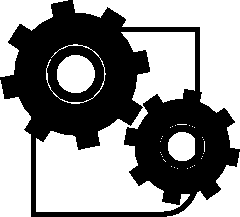
\includegraphics[width=0.75cm]{col11305.imgs/summary_simulation.png} &   \end{array} $ \hspace{2 pt}\raisebox{-5 pt}{} {(section shortcode: P10022 )} \par 
The chemical properties of an element depend on the number of protons and electrons inside the atom. So if a neutron or two is added or removed from the nucleus, then the chemical properties will not change. This means that such an atom would remain in the same place in the periodic table. For example, no matter how many neutrons we add or subtract from a nucleus with 6 protons, that element will \textbf{always} be called carbon and have the element symbol $\text{C}$ (see the periodic table). Atoms which have the same number of protons (i.e.\@{} same atomic number $Z$), but a different number of neutrons (i.e.\@{} different $N$ and therefore different mass number $A$), are called \textbf{isotopes}. 

\IFact{In Greek, ``same place'' reads as $\stackrel{`}{\iota }\sigma o\varsigma \tau \stackrel{`}{o}\pi o\varsigma $\hspace{1ex} (isos topos). This is why atoms which have the same number of protons, but different numbers of neutrons, are called \textsl{isotopes}. They are in the same place on the periodic table!}

\Definition{  Isotope } { Isotopes of an element have the same number of protons (same $Z$), but a different number of neutrons (different $N$).} 

\label{m38753*id257405} The chemical properties of the different isotopes of an element are the same, but they might vary in how stable their nucleus is. We can also write elements as $\text{E - A}$ where the E is the element symbol and the A is the atomic mass of that element. For example $\text{Cl-}35$ has an atomic mass of $35 \text{ u}$ ($17$ protons and \textbf{$18$ neutrons}), while $\text{Cl-}37$ has an atomic mass of $37 \text{ u}$ ($17$ protons and \textbf{$20$ neutrons}).\\

\label{m38753*id248557}In nature the different isotopes occur in different percentages. For example $\text{Cl-}35$ might make up $75\%$ of all chlorine atoms on Earth, and $\text{Cl-}37$ makes up the remaining $25\%$. The following worked example will show you how to calculate the average atomic mass for these two isotopes:    
\begin{wex}{The relative atomic mass of an isotopic element}{
The element chlorine has two isotopes, $\text{chlorine-}35$ and $\text{chlorine-}37$. The abundance of these isotopes when they occur naturally is $75\% \text{ chlorine-}35$ and $25\% \text{ chlorine-}37$. Calculate the \textit{average} relative atomic mass for chlorine.
}
{
\westep{Calculate the mass contribution of chlorine-$35$ to the average relative atomic mass}
$75\%$ of the chlorine atoms has a mass of of $35 \text{ u}$ \\
Contribution of $\text{Cl-}35 = (\frac{75}{100} \times 35) = 26,25~\text{u}$

\westep{Calculate the contribution of chlorine-$37$ to the average relative atomic mass}
$25\%$ of the chlorine atoms has a mass of of $37 \text{ u}$ \\ 
Contribution of $\text{Cl-}37 = (\frac{25}{100} \times 37) = 9,25 \text{ u}$


\westep{Add the two values to arrive at the \textit{average relative atomic mass} of chlorine}

$\text{Relative atomic mass of chlorine} = 26,25\text{ u} + 9,25\text{ u} = 35,5\text{ u}$ \\
}
\end{wex}
If you look on the periodic table (see front of book), the average relative atomic mass for chlorine is $35,5 \text{ u}$. \simulation{PhET simulation for Isotopes}{VPcyv}
\clearpage

% \label{m38753*secfhsst!!!underscore!!!id567}
% \par \practiceinfo
%  \par \begin{tabular}[h]{cccccc}
%  (1.) 000u  &  (2.) 000v  &  (3.) 000w  & \end{tabular}
   \begin{exercises}  {Isotopes }
            \nopagebreak \noindent \vspace{-2cm}
        \label{m38753*id258162}\begin{enumerate}[noitemsep, label=\textbf{\arabic*}. ] 
%Question 1
            \label{m38753*uid50}\item Atom A has $5$ protons and $5$ neutrons, and atom B has $6$ protons and $5$ neutrons. These atoms are:
\label{m38753*id258178}\begin{enumerate}[noitemsep, label=\textbf{\alph*}. ] 
            \label{m38753*uid51}\item allotropes
\label{m38753*uid52}\item isotopes
\label{m38753*uid53}\item isomers
\label{m38753*uid54}\item atoms of different elements
\end{enumerate}
%Question 2
                \label{m38753*uid55}\item For the sulphur isotopes, $_{16}^{32}\text{S}$ and $_{16}^{34}\text{S}$, give the number of:
\label{m38753*id258277}\begin{enumerate}[noitemsep, label=\textbf{\alph*}. ] 
            \label{m38753*uid56}\item protons
\label{m38753*uid57}\item nucleons
\label{m38753*uid58}\item electrons
\label{m38753*uid59}\item neutrons
\end{enumerate}
%Question 3
                \label{m38753*uid60}\item Which of the following are isotopes of $_{17}^{35}\text{Cl}$?
\label{m38753*id258355}\begin{enumerate}[noitemsep, label=\textbf{\alph*}. ] 
            \label{m38753*uid61}\item $_{35}^{17}\text{Cl}$
\label{m38753*uid62}\item $_{17}^{35}\text{Cl}$
\label{m38753*uid63}\item $_{17}^{37}\text{Cl}$
\end{enumerate}
%Question 4
                \label{m38753*uid64}\item Which of the following are isotopes of $\text{U-}235$? (E represents an element symbol)
\label{m38753*id258452}\begin{enumerate}[noitemsep, label=\textbf{\alph*}. ] 
            \label{m38753*uid65}\item $_{92}^{238}\text{E}$
\label{m38753*uid66}\item $_{90}^{238}\text{E}$
\label{m38753*uid67}\item $_{92}^{235}\text{E}$
\end{enumerate}
%Question 5
            \label{m38753*uid619}\item Complete the table below:
    % \textbf{m38753*id25871115}\par
          \begin{center}
\begin{tabular}{|p{2cm}|p{1cm}|p{1cm}|p{1.4cm}|p{1.4cm}|p{1.4cm}|}\hline
\textbf{Isotope} & \textbf{Z} & \textbf{A} & \textbf{Protons} & \textbf{Neutrons} & \textbf{Electrons}\\\hline
Carbon-$12$ & & & & & \\\hline
Carbon-$14$ & & & & & \\\hline
Iron-$54$ & & & & & \\\hline
Iron-$56$ & & & & & \\\hline
Iron-$57$ & & & & & \\ \hline
\end{tabular}
\end{center}
%Question 6
\item If a sample contains $19,9\%$ boron-$10$ and $80,1\%$ boron-$11$, calculate the relative atomic mass of an atom of boron in that sample.
\hspace{1ex}    
%Question 7    
\label{m38753*uid7100}\item If a sample contains $79\% \text{ Mg-}24$, $10\% \text{ Mg-}25$ and $11\% \text{ Mg-}26$, calculate the relative atomic mass of an atom of magnesium in that sample.
%Question 8
\item For the element $^{234}_{92}{\text{U}}$ (uranium), use standard notation to describe:
\begin{enumerate}[noitemsep, label=\textbf{\alph*}. ]
 \item the isotope with $2$ fewer neutrons
 \item the isotope with $4$ more neutrons
\end{enumerate}
%Question 9
\item Which of the following are isotopes of $^{40}_{20}\text{Ca}$?
\begin{enumerate}[noitemsep, label=\textbf{\alph*}. ]
 \item $^{40}_{19}\text{K}$
 \item $^{42}_{20}\text{Ca}$
 \item $^{40}_{18}\text{Ar}$
\end{enumerate}
%Question 10
\item For the sulphur isotope $^{33}_{16}\text{S}$, give the number of:
	\begin{enumerate}[noitemsep, label=\textbf{\alph*}. ]
	\item{protons}
	\item{nucleons}
	\item{electrons}
	\item{neutrons}
	\end{enumerate}
\hspace{1ex}        
                \end{enumerate}
      \label{m38753*uid68}
\practiceinfo
\par 
 \par \begin{tabular}[h]{ccccc}
 (1.) 000x  &  (2.) 000y  &  (3.) 000z  &  (4.) 0010  & (5.) 0011 
(6.) 0012  & (7.) 0013 & (8.) 0014 & (9.) 0015 & (10.) 0016 
\end{tabular}

\end{exercises}

         \section{Electronic configuration}
    \nopagebreak
%            \label{m38741} $ \hspace{-5pt}\begin{array}{cccccccccccc}   
\includegraphics[width=0.75cm]{col11305.imgs/summary_fullmarks.png} &   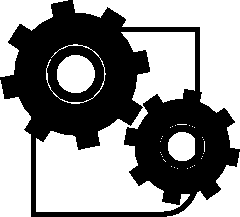
\includegraphics[width=0.75cm]{col11305.imgs/summary_simulation.png} &   
\includegraphics[width=0.75cm]{col11305.imgs/summary_video.png} &   
\includegraphics[width=0.75cm]{col11305.imgs/summary_presentation.png} &   \end{array} $ \hspace{2 pt}\raisebox{-5 pt}{} {(section shortcode: P10023 )} \par 
    \label{m38741*cid7}
            \nopagebreak
      \label{m38741*uid79}
            \subsection*{The energy of electrons}
            \nopagebreak
        \label{m38741*id259210}The electrons of an atom all have the same charge and the same mass, but each electron has a different amount of \textsl{energy}. Electrons that have the \textsl{lowest} energy are found closest to the nucleus (where the attractive force of the positively charged nucleus is the greatest) and the electrons that have \textsl{higher} energy (and are able to overcome the attractive force of the nucleus) are found further away.\\
\mindsetvid{quantisation}{VPama}
      \label{m38741*uid81}
            \subsection*{Electron arrangement}
            \nopagebreak
            \label{m38741*id9722401}We will start with a very simple view of the arrangement or configuration of electrons around an atom. This view simply states that electrons are arranged in energy levels (or shells) around the nucleus of an atom. These energy levels are numbered $1$, $2$, $3$, etc. Electrons that are in the first energy level (energy level $1$) are closest to the nucleus and will have the lowest energy. Electrons further away from the nucleus will have a higher energy. \par 
\label{m38741*id259357}In the following examples, the energy levels are shown as concentric circles around the central nucleus. The important thing to know for these diagrams is that the first energy level can hold 2 electrons, the second energy level can hold $8$ electrons and the third energy level can hold $8$ electrons.\pagebreak 
\begin{enumerate}[noitemsep, label=\textbf{\arabic*}. ] 

\item{\textbf{Lithium} \\
\begin{minipage}{.4\textwidth}
Lithium ($\text{Li}$) has an atomic number of $3$, meaning that in a neutral atom, the number of electrons will also be $3$. The first two electrons are found in the first energy level, while the third electron is found in the second energy level (Figure~\ref{fig:atom:lithium}).
\end{minipage}
\begin{minipage}{.6\textwidth}
\begin{figure}[H]
\begin{center}
\scalebox{.7}{
\begin{pspicture}(-5,1)(7,4)
\SpecialCoor
%\psgrid[gridcolor=lightgray]
\rput(0,3){
\pscircle(0,0){1.25}
\pscircle(0,0){0.75}
\pscircle[fillcolor=lightgray,fillstyle=solid](0,0){0.25}
\multido{\n=90+180}{2}{\pscircle[fillcolor=black,fillstyle=solid]({0.75;\n}){0.1}}
\pscircle[fillcolor=black,fillstyle=solid]({1.25;0}){0.1}
\psline(2,0.8)(0.9,0.8)
\uput[r](2,0.8){second energy level}
\psline(2,-0.4)(0.6,-0.4)
\uput[r](2,-0.4){first energy level}
\psline(2,0)({0.75;90})
\psline(2,0)({1.25;0})
\uput[r](2,0){electrons}
\psline({0.25;-45})(0.8,-1.2)(2,-1.2)
\uput[r](2,-1.2){\parbox[l]{4cm}{nucleus, containing 3 protons and 4 neutrons}}
}
\end{pspicture}
}
\caption{Electron arrangement of a lithium atom.}
\label{fig:atom:lithium}
\end{center}
\end{figure}
\end{minipage}
}

\item{\textbf{Fluorine} \\
\begin{minipage}{.4\textwidth}
Fluorine ($\text{F}$) has an atomic number of $9$, meaning that a neutral atom also has $9$ electrons. The first $2$ electrons are found in the first energy level, while the other $7$ are found in the second energy level (Figure~\ref{fig:atom:fluorine}).
\end{minipage}
\begin{minipage}{.6\textwidth}
\begin{figure}[H]
\begin{center}
\scalebox{1}{
\begin{pspicture}(-5.5,-2)(7,1.5)
\pscircle(0,0){1.25}
\pscircle(0,0){0.75}
\pscircle[fillcolor=lightgray,fillstyle=solid](0,0){0.25}
\multido{\n=90+180}{2}{\pscircle[fillcolor=black,fillstyle=solid]({0.75;\n}){0.1}}
\multido{\n=0+45}{7}{\pscircle[fillcolor=black,fillstyle=solid]({1.25;\n}){0.1}}
\end{pspicture}
}
\caption{Electron arrangement of a fluorine atom.}
\label{fig:atom:fluorine}
\end{center}
\end{figure}
\end{minipage}
}

\item{\textbf{Neon} \\
\begin{minipage}{.4\textwidth}
Neon ($\text{Ne}$) has an atomic number of $10$, meaning that a neutral atom also has $10$ electrons. The first $2$ electrons are found in the first energy level and the last $8$ are found in the second energy level. (Figure~\ref{fig:atom:neon}).
\end{minipage}
\begin{minipage}{.6\textwidth}
\begin{figure}[H]
\begin{center}
\scalebox{1.2}{
\begin{pspicture}(-6,-2)(7,2)
% \pscircle(0,0){1.75}
\pscircle(0,0){1.25}
\pscircle(0,0){0.75}
\pscircle[fillcolor=lightgray,fillstyle=solid](0,0){0.25}
\multido{\n=90+180}{2}{\pscircle[fillcolor=black,fillstyle=solid]({0.75;\n}){0.1}}
\multido{\n=0+45}{8}{\pscircle[fillcolor=black,fillstyle=solid]({1.25;\n}){0.1}}
% \multido{\n=0+45}{8}{\pscircle[fillcolor=black,fillstyle=solid]({1.75;\n}){0.1}}
\pscircle[fillcolor=black,fillstyle=solid]({1.25;0}){0.1}
\end{pspicture}
}
\caption{Electron arrangement of a neon atom.}
\label{fig:atom:neon}
\end{center}
\end{figure}
\end{minipage}
}
\end{enumerate}

But the situation is slightly more complicated than this. Within each energy level, the electrons move in \textbf{orbitals}. An orbital defines the spaces or regions where electrons move.

\Definition{ Atomic orbital} {An atomic orbital is the region in which an electron may be found around a single atom.} 

The first energy level contains only one s orbital, the second energy level contains one s orbital and three p orbitals and the third energy level contains one s orbital and three p orbitals (as well as five d orbitals). Within each energy level, the s orbital is at a lower energy than the p orbitals. This arrangement is shown in Figure~\ref{fig:Aufbau:blank}. 

\begin{figure}[H]
\begin{center}
 \scalebox{.6}{
 \begin{pspicture}(-6,-8)(6,5)
%\psgrid
 
\rput(-4,0){
% 1s
  \rput(0,-6){ \scalebox{0.5}{	\pspolygon(0,0)(0,2)(3,2)(3,0) }
	\uput[ur](0,1){1s} }
% 2s
  \rput(0,-3){ \scalebox{0.5}{	\pspolygon(0,0)(0,2)(3,2)(3,0) }
	\uput[ur](0,1){2s} }
% 3s
  \rput(0,0){ \scalebox{0.5}{	\pspolygon(0,0)(0,2)(3,2)(3,0) }
	\uput[ur](0,1){3s} }
% 4s
  \rput(0,3){ \scalebox{0.5}{	\pspolygon(0,0)(0,2)(3,2)(3,0) }
	\uput[ur](0,1){4s} }
% 2p
  \rput(2,-2){ \scalebox{0.5}{	\pspolygon(0,0)(0,2)(3,2)(3,0) }
	\uput[ur](0,1){2p} }
  \rput(3.5,-2){ \scalebox{0.5}{	\pspolygon(0,0)(0,2)(3,2)(3,0) }}
  \rput(5,-2){ \scalebox{0.5}{\pspolygon(0,0)(0,2)(3,2)(3,0) }}
% 3p
  \rput(2,1){ \scalebox{0.5}{	\pspolygon(0,0)(0,2)(3,2)(3,0) }	
	\uput[ur](0,1){3p} }
  \rput(3.5,1){ \scalebox{0.5}{\pspolygon(0,0)(0,2)(3,2)(3,0) }}
  \rput(5,1){ \scalebox{0.5}{	\pspolygon(0,0)(0,2)(3,2)(3,0) }}

  \psline(-0.5,-7)(-0.5,5)
  \uput[dr](-2,-1.5){  \scalebox{1.5}{\parbox{\linewidth}{E \\ N \\ E \\ R \\ G \\ Y}} }  
  \uput[u](-1.55,-1){ \psline[doubleline=true, doublesep=3pt]{->}(0,0)(0,3) }

\rput(0,0.5){
\psline(-0.5,-4.25)(7.5,-2.75)
\psline(-0.5,-1.25)(7.5,0.25)
\psline(-0.5,1.75)(7.5,3.25)

\uput[ur](7,-5){ \parbox{\linewidth}{First main \\ energy level} }
\uput[ur](7,-2){ \parbox{\linewidth}{Second main \\ energy level} }
\uput[ur](7,1){ \parbox{\linewidth}{Third main \\ energy level} }
}
}
\end{pspicture}
}
\end{center}
\caption{The positions of the first ten orbitals of an atom on an energy diagram.}
\label{fig:Aufbau:blank}
\end{figure}

\Note{Each block in figure~\ref{fig:Aufbau:blank} is able to hold two electrons. This means that the s orbital can hold two electrons, while the p orbital can hold a total of six electrons, two in each of the three blocks.}

\label{m38741*eip-752}This diagram also helps us when we are working out the electron configuration of an element. The electron configuration of an element is the arrangement of the electrons in the shells and subshells. There are a few guidelines for working out the electron configuration. These are:
\label{m38741*id259303}\begin{itemize}[noitemsep]
            \label{m38741*uid93}\item Each orbital can only hold \textbf{two electrons}. Electrons that occur together in an orbital are called an \textbf{electron pair}.
\label{m38741*uid94}\item An electron will always try to enter an orbital with the lowest possible energy.
\label{m38741*uid95}\item An electron will occupy an orbital on its own, rather than share an orbital with another electron. An electron would also rather occupy a lower energy orbital \textsl{with} another electron, before occupying a higher energy orbital. In other words, within one energy level, electrons will fill an s orbital before starting to fill p orbitals.
\label{m38741*uid83}\item The s subshell can hold 2 electrons
\label{m38741*uid84}\item The p subshell can hold 6 electrons
\end{itemize}
        \label{m38741*id259599}The way that the electrons are arranged in an atom is called its \textbf{electron configuration}.
\Tip{When there are two electrons in an orbital, the electrons are called an \textbf{electron pair}. If the orbital only has one electron, this electron is said to be an \textbf{unpaired electron}. Electron pairs are shown with arrows pointing in opposite directions.}
        

\Definition{ Electron configuration }{Electron configuration is the arrangement of electrons in an atom, molecule or other physical structure.} 
\subsection*{Aufbau diagrams}        
\label{m38741*id259628}An element's electron configuration can be represented using \textbf{Aufbau diagrams} or energy level diagrams. An Aufbau diagram uses arrows to represent electrons. You can use the following steps to help you to draw an Aufbau diagram:
        \label{m38741*id259639}\begin{enumerate}[noitemsep, label=\textbf{\arabic*}. ] 
\item Determine the number of electrons that the atom has.
\item Fill the s orbital in the first energy level (the $1\text{s}$ orbital) with the first two electrons.
\item Fill the s orbital in the second energy level (the $2\text{s}$ orbital) with the second two electrons.
\item Put one electron in each of the three p orbitals in the second energy level (the $2\text{p}$ orbitals) and then if there are still electrons remaining, go back and place a second electron in each of the $2\text{p}$ orbitals to complete the electron pairs.
\item Carry on in this way through each of the successive energy levels until all the electrons have been drawn.
\end{enumerate}
\IFact{Aufbau is the German word for ``building up''. Scientists used this term since this is exactly what we are doing when we work out electron configuration, we are building up the atoms structure.}


\label{m38741*eip-873}You can think of Aufbau diagrams as being similar to people getting on a bus or a train. People will first sit in empty seats with empty seats between them and the other people (unless they know the people and then they will sit next to them). This is the lowest energy. When all the seats are filled like this, any more people that get on will be forced to sit next to someone. This is higher in energy. As the bus or train fills even more the people have to stand to fit on. This is the highest energy.  \label{m38741*id259728}
            \subsubsection*{Hund's rule and Pauli's principle}
            \nopagebreak
            \label{m38741*eip-188}
Sometimes people refer to Hund's rule for electron configuration. This rule simply says that electrons would rather be in a subshell on their own than share a subshell. This is why when you are filling the subshells you put one electron in each subshell and then go back and fill the subshell, before moving onto the next energy level.
\par 
\label{m38741*eip-id1167385514309}
Pauli's exclusion principle simply states that electrons have a property known as spin and that two electrons in a subshell will not spin the same way. This is why we draw electrons as one arrow pointing up and one arrow pointing down.
\par \label{m38741*uid104}
\subsection*{Spectroscopic electron configuration notation}
        \label{m38741*id259749}A special type of notation is used to show an atom's electron configuration. The notation describes the energy levels, orbitals and the number of electrons in each. For example, the electron configuration of lithium is ${1\text{s}}^{2}{2\text{s}}^{1}$. The number and letter describe the energy level and orbital and the number above the orbital shows how many electrons are in that orbital. 

Aufbau diagrams for the elements fluorine and argon are shown in Figures~\ref{fig:Aufbau:fluorine} and \ref{fig:Aufbau:argon} respectively. Using spectroscopic notation, the electron configuration of fluorine is $1\text{s}^{2}{2}\text{s}^{2}2\text{p}^{5}$ and the electron configuration of argon is $1\text{s}^{2}{2}\text{s}^{2}2\text{p}^{5}{3}\text{s}^{2}3\text{p}^{6}$. \\
\Tip{The spectroscopic electron configuration can be written in shorter form. This form is written as [noble gas]electrons, where the noble gas is the nearest one that occurs before the element. For example, magnesium can be represented as $\text{[Ne]}3\text{s}^{2}$ and carbon as $\text{[H]}2\text{s}^{2}2\text{p}^{2}$. This is known as the condensed electron configuration.}
% \begin{minipage}{.45\textwidth}
\begin{multicols}{2}
\begin{figure}[H]
\begin{center}
\scalebox{0.7}{
\begin{pspicture}(-8,-8)(8,5)
%\psgrid
 
 \newpsobject{spin}{psline}{arrowsize=10pt, arrowinset=0, linewidth=3pt}

% 1s
  \rput(0,-5){ \scalebox{0.5}{	\pspolygon(0,0)(0,2)(3,2)(3,0) 
  	\spin{->}(1,0.2)(1,1.8)	\spin{->}(2,1.8)(2,0.2) }
	\uput[ur](0,1){1s} }
% 2s
  \rput(0,-3){ \scalebox{0.5}{	\pspolygon(0,0)(0,2)(3,2)(3,0) 
	\spin{->}(1,0.2)(1,1.8)	\spin{->}(2,1.8)(2,0.2) }
	\uput[ur](0,1){2s} }
% 3s
\rput(0,0){ \scalebox{0.5}{ \pspolygon(0,0)(0,2)(3,2)(3,0) }
	\uput[ur](0,1){3s} }
% 2p
  \rput(2,-2){ \scalebox{0.5}{	\pspolygon(0,0)(0,2)(3,2)(3,0) 
	\spin{->}(1,0.2)(1,1.8)	\spin{->}(2,1.8)(2,0.2) } 
	\uput[ur](0,1){2p} }
  \rput(3.5,-2){ \scalebox{0.5}{	\pspolygon(0,0)(0,2)(3,2)(3,0) 
	\spin{->}(1,0.2)(1,1.8)	\spin{->}(2,1.8)(2,0.2) } }
  \rput(5,-2){ \scalebox{0.5}{\pspolygon(0,0)(0,2)(3,2)(3,0) 	\spin{->}(1,0.2)(1,1.8)}}
% 3p
\rput(2,1){ \scalebox{0.5}{\pspolygon(0,0)(0,2)(3,2)(3,0)}
	\uput[ur](0,1){3p} }
\rput(3.5,1){ \scalebox{0.5}{\pspolygon(0,0)(0,2)(3,2)(3,0)}}
\rput(5,1){ \scalebox{0.5}{ \pspolygon(0,0)(0,2)(3,2)(3,0)}}
\end{pspicture}
}

\caption{An Aufbau diagram showing \\ the electron configuration of fluorine}
\label{fig:Aufbau:fluorine}
\end{center}
\end{figure}
% \end{minipage}


% \begin{minipage}{.45\textwidth}

\begin{figure}[H]
\begin{center}
\scalebox{0.7}{
\begin{pspicture}(-8,-7)(8,4)
%\psgrid
\newpsobject{spin}{psline}{arrowsize=10pt, arrowinset=0, linewidth=3pt}

\rput(-2,0){
% 1s
\rput(0,-5){ \scalebox{0.5}{	\pspolygon(0,0)(0,2)(3,2)(3,0) 
	\spin{->}(1,0.2)(1,1.8)	\spin{->}(2,1.8)(2,0.2) 	}
	\uput[ur](0,1){1s} }
% 2s
\rput(0,-3){ \scalebox{0.5}{	\pspolygon(0,0)(0,2)(3,2)(3,0) 
	\spin{->}(1,0.2)(1,1.8)	\spin{->}(2,1.8)(2,0.2) 	}
	\uput[ur](0,1){2s} }
% 3s
\rput(0,0){ \scalebox{0.5}{		\pspolygon(0,0)(0,2)(3,2)(3,0) 
	\spin{->}(1,0.2)(1,1.8)	\spin{->}(2,1.8)(2,0.2) 	}
	\uput[ur](0,1){3s} }
% 2p
\rput(2,-2){ \scalebox{0.5}{	\pspolygon(0,0)(0,2)(3,2)(3,0) 
	\spin{->}(1,0.2)(1,1.8)	\spin{->}(2,1.8)(2,0.2)	}
	\uput[ur](0,1){2p} }
\rput(3.5,-2){ \scalebox{0.5}{	\pspolygon(0,0)(0,2)(3,2)(3,0) 
	\spin{->}(1,0.2)(1,1.8)	\spin{->}(2,1.8)(2,0.2)	} 	}
\rput(5,-2){ \scalebox{0.5}{	\pspolygon(0,0)(0,2)(3,2)(3,0) 
	\spin{->}(1,0.2)(1,1.8)	\spin{->}(2,1.8)(2,0.2)	}	}
% 3p
\rput(2,1){ \scalebox{0.5}{		\pspolygon(0,0)(0,2)(3,2)(3,0) 
	\spin{->}(1,0.2)(1,1.8)	\spin{->}(2,1.8)(2,0.2)	}
	\uput[ur](0,1){3p} }
\rput(3.5,1){ \scalebox{0.5}{	\pspolygon(0,0)(0,2)(3,2)(3,0) 
	\spin{->}(1,0.2)(1,1.8)	\spin{->}(2,1.8)(2,0.2)	}	}
\rput(5,1){ \scalebox{0.5}{		\pspolygon(0,0)(0,2)(3,2)(3,0) 
	\spin{->}(1,0.2)(1,1.8)	\spin{->}(2,1.8)(2,0.2)	}	}
}
\end{pspicture}
}

\caption{An Aufbau diagram showing \\ the electron configuration of argon}
\label{fig:Aufbau:argon}
\end{center}
\end{figure}
\end{multicols}
% \end{minipage}

\begin{wex}
{%title
Aufbau diagrams and spectroscopic electron configuration 
}
{%question
Give the electron configuration for nitrogen ($\text{N}$) and draw an Aufbau diagram.
}
{%answer
\westep{Give the number of electrons} Nitrogen has seven electrons.
\westep{Place two electrons in the $1\text{s}$ orbital} We start by placing two electrons in the $1\text{s}$ orbital: ${1\text{s}}^{2}$. 
\begin{figure}[H]
\scalebox{0.7}{
 \begin{pspicture}(-8,-6)(8,-2)
%\psgrid
\pspolygon[lincolor=black,fillstyle=solid,fillcolor=white](-2.5,-5.5)(-2.5,-3.2)(0,-3.2)(0,-5.5)
 \newpsobject{spin}{psline}{arrowsize=10pt, arrowinset=0, linewidth=3pt}
\rput(-2,0){
  \rput(0,-5){ \scalebox{0.5}{	\pspolygon(0,0)(0,2)(3,2)(3,0) 
  	\spin{->}(1,0.2)(1,1.8)	\spin{->}(2,1.8)(2,0.2) }
	\uput[ur](0,1){1s} }
}
\end{pspicture}
}
\label{fig:Aufbau:wex}
\end{figure}
Now we have five electrons left to place in orbitals.  
\westep{Place two electrons in the $2\text{s}$ orbital} 
We put two electrons in the $2\text{s}$ orbital: ${2\text{s}}^{2}$. 
%     \setcounter{subfigure}{0}
\begin{figure}[H]
\scalebox{0.7}{
 \begin{pspicture}(-8,-6)(8,-2)
%\psgrid
\pspolygon[lincolor=black,fillstyle=solid,fillcolor=white](-2.5,-5.5)(-2.5,-1.2)(0,-1.2)(0,-5.5)
 \newpsobject{spin}{psline}{arrowsize=10pt, arrowinset=0, linewidth=3pt}
\rput(-2,0){
% 1s
  \rput(0,-5){ \scalebox{0.5}{	\pspolygon(0,0)(0,2)(3,2)(3,0) 
  	\spin{->}(1,0.2)(1,1.8)	\spin{->}(2,1.8)(2,0.2) }
	\uput[ur](0,1){1s} }
% 2s
  \rput(0,-3){ \scalebox{0.4}{	\pspolygon(0,0)(0,2)(3,2)(3,0) 
	\spin{->}(1,0.2)(1,1.8)	\spin{->}(2,1.8)(2,0.2) }
	\uput[ur](0,1){2s} }
}
\end{pspicture}
}
\label{fig:Aufbau:wex1}
\end{figure}    
There are now three electrons to place in orbitals.
\westep{Place three electrons in the $2\text{p}$ orbital}
We place three electrons in the $2\text{p}$ orbital: ${2\text{p}}^{3}$.
\begin{figure}[H]
\scalebox{.7}{
 \begin{pspicture}(-8,-8)(8,5)
%\psgrid
\pspolygon[lincolor=black,fillstyle=solid,fillcolor=white](-4.5,-5.5)(-4.5,0)(14,0)(14,-5.5) 
 \newpsobject{spin}{psline}{arrowsize=10pt, arrowinset=0, linewidth=3pt}
%1st p electron
\rput(-4,0){
% 1s
  \rput(0,-5){ \scalebox{0.4}{	\pspolygon(0,0)(0,2)(3,2)(3,0) 
  	\spin{->}(1,0.2)(1,1.8)	\spin{->}(2,1.8)(2,0.2) }
	\uput[ur](0,1){1s} }
% 2s
  \rput(0,-3){ \scalebox{0.4}{	\pspolygon(0,0)(0,2)(3,2)(3,0) 
	\spin{->}(1,0.2)(1,1.8)	\spin{->}(2,1.8)(2,0.2) }
	\uput[ur](0,1){2s} }
% 2p
  \rput(1.8,-2){ \scalebox{0.4}{\pspolygon(0,0)(0,2)(3,2)(3,0) 
	\spin{->}(1,0.2)(1,1.8)	 } 
	\uput[ur](0,1){2p} }
  \rput(3,-2){ \scalebox{0.4}{ \pspolygon(0,0)(0,2)(3,2)(3,0) 
		 } }
  \rput(4.2,-2){ \scalebox{0.4}{\pspolygon(0,0)(0,2)(3,2)(3,0) }}}
%second p electron
\rput(2,0){
% 1s
  \rput(0,-5){ \scalebox{0.4}{	\pspolygon(0,0)(0,2)(3,2)(3,0) 
  	\spin{->}(1,0.2)(1,1.8)	\spin{->}(2,1.8)(2,0.2) }
	\uput[ur](0,1){1s} }
% 2s
  \rput(0,-3){ \scalebox{0.4}{	\pspolygon(0,0)(0,2)(3,2)(3,0) 
	\spin{->}(1,0.2)(1,1.8)	\spin{->}(2,1.8)(2,0.2) }
	\uput[ur](0,1){2s} }
% 2p
  \rput(1.8,-2){ \scalebox{0.4}{\pspolygon(0,0)(0,2)(3,2)(3,0) 
	\spin{->}(1,0.2)(1,1.8)	 } 
	\uput[ur](0,1){2p} }
  \rput(3,-2){ \scalebox{0.4}{ \pspolygon(0,0)(0,2)(3,2)(3,0) 
	\spin{->}(1,0.2)(1,1.8)	 } }
  \rput(4.2,-2){ \scalebox{0.4}{\pspolygon(0,0)(0,2)(3,2)(3,0) }}}
%3rd p electron
\rput(8,0){
% 1s
  \rput(0,-5){ \scalebox{0.4}{	\pspolygon(0,0)(0,2)(3,2)(3,0) 
  	\spin{->}(1,0.2)(1,1.8)	\spin{->}(2,1.8)(2,0.2) }
	\uput[ur](0,1){1s} }
% 2s
  \rput(0,-3){ \scalebox{0.4}{	\pspolygon(0,0)(0,2)(3,2)(3,0) 
	\spin{->}(1,0.2)(1,1.8)	\spin{->}(2,1.8)(2,0.2) }
	\uput[ur](0,1){2s} }
% 2p
  \rput(1.8,-2){ \scalebox{0.4}{\pspolygon(0,0)(0,2)(3,2)(3,0) 
	\spin{->}(1,0.2)(1,1.8)	 } 
	\uput[ur](0,1){2p} }
  \rput(3,-2){ \scalebox{0.4}{ \pspolygon(0,0)(0,2)(3,2)(3,0) 
	\spin{->}(1,0.2)(1,1.8)	 } }
  \rput(4.2,-2){ \scalebox{0.4}{\pspolygon(0,0)(0,2)(3,2)(3,0) \spin{->}(1,0.2)(1,1.8) }}
}
\end{pspicture}
}
\label{fig:Aufbau:wex2}
\end{figure}
\westep{Write the final answer} The electron configuration is: ${1\text{s}}^{2}{2\text{s}}^{2}{2\text{p}}^{3}$. The Aufbau diagram is given in the step above.
  
} 
\end{wex} 
\subsubsection*{Aufbau diagrams for ions}
When a neutral atom loses an electron it becomes positively charged and we call it a cation. For example, sodium will lose one electron and become $\text{Na}^{+}$ or calcium will lose two electrons and become $\text{Ca}^{2+}$. In each of these cases, the outermost electron(s) will be lost. \\
When a neutral atom gains an electron it becomes negatively charged and we call it an anion. For example chlorine will gain one electron and become $\text{Cl}^{-}$ or oxygen will gain two electrons and become $\text{O}^{2-}$.  \\
Aufbau diagrams and electron configurations can be done for cations and anions as well. The following worked example will show you how. \\


\begin{wex}
{%title
Aufbau diagram for an ion
}
{%question
Give the electron configuration for ($\text{O}^{2-}$) and draw an Aufbau diagram.
}
{%answer
\westep{Give the number of electrons} Oxygen has eight electrons. The oxygen anion has gained two electrons and so the total number of electrons is ten.
\westep{Place two electrons in the $1\text{s}$ orbital} We start by placing two electrons in the $1\text{s}$ orbital: ${1\text{s}}^{2}$. 
\begin{figure}[H]
\scalebox{0.7}{
 \begin{pspicture}(-8,-6)(8,-2)
%\psgrid
\pspolygon[lincolor=black,fillstyle=solid,fillcolor=white](-2.5,-5.5)(-2.5,-3.2)(0,-3.2)(0,-5.5)
 \newpsobject{spin}{psline}{arrowsize=10pt, arrowinset=0, linewidth=3pt}
\rput(-2,0){
  \rput(0,-5){ \scalebox{0.5}{	\pspolygon(0,0)(0,2)(3,2)(3,0) 
  	\spin{->}(1,0.2)(1,1.8)	\spin{->}(2,1.8)(2,0.2) }
	\uput[ur](0,1){1s} }
}
\end{pspicture}
}
\label{fig:Aufbau:wex}
\end{figure}
Now we have eight electrons left to place in orbitals.  
\westep{Place two electrons in the $2\text{s}$ orbital} 
We put two electrons in the $2\text{s}$ orbital: ${2\text{s}}^{2}$. 
    \setcounter{subfigure}{0}
\begin{figure}[H]
\scalebox{0.7}{
 \begin{pspicture}(-8,-6)(8,-2)
%\psgrid
\pspolygon[lincolor=black,fillstyle=solid,fillcolor=white](-2.5,-5.5)(-2.5,-1.2)(0,-1.2)(0,-5.5)
 \newpsobject{spin}{psline}{arrowsize=10pt, arrowinset=0, linewidth=3pt}
\rput(-2,0){
% 1s
  \rput(0,-5){ \scalebox{0.5}{	\pspolygon(0,0)(0,2)(3,2)(3,0) 
  	\spin{->}(1,0.2)(1,1.8)	\spin{->}(2,1.8)(2,0.2) }
	\uput[ur](0,1){1s} }
% 2s
  \rput(0,-3){ \scalebox{0.5}{	\pspolygon(0,0)(0,2)(3,2)(3,0) 
	\spin{->}(1,0.2)(1,1.8)	 }
	\uput[ur](0,1){2s} }
}
\end{pspicture}
}
\label{fig:Aufbau:wex1}
\end{figure}    
There are now six electrons to place in orbitals.
\westep{Place six electrons in the $2\text{p}$ orbital}
We place six electrons in the $2\text{p}$ orbital: ${2\text{p}}^{6}$.
\westep{Write the final answer} The electron configuration is: ${1\text{s}}^{2}{2\text{s}}^{2}{2\text{p}}^{6}$. The Aufbau diagram is:
\begin{figure}[H]
\scalebox{.7}{
 \begin{pspicture}(-8,-8)(8,5)
%\psgrid
\pspolygon[lincolor=black,fillstyle=solid,fillcolor=white](-2.5,-5.5)(-2.5,0)(5,0)(5,-5.5) 
 \newpsobject{spin}{psline}{arrowsize=10pt, arrowinset=0, linewidth=3pt}
\rput(-2,0){
% 1s
  \rput(0,-5){ \scalebox{0.5}{	\pspolygon(0,0)(0,2)(3,2)(3,0) 
  	\spin{->}(1,0.2)(1,1.8)	\spin{->}(2,1.8)(2,0.2) }
	\uput[ur](0,1){1s} }
% 2s
  \rput(0,-3){ \scalebox{0.5}{	\pspolygon(0,0)(0,2)(3,2)(3,0) 
	\spin{->}(1,0.2)(1,1.8)	\spin{->}(2,1.8)(2,0.2) }
	\uput[ur](0,1){2s} }
% 2p
  \rput(2,-2){ \scalebox{0.5}{	\pspolygon(0,0)(0,2)(3,2)(3,0) 
	\spin{->}(1,0.2)(1,1.8)	\spin{->}(2,1.8)(2,0.2) } 
	\uput[ur](0,1){2p} }
  \rput(3.5,-2){ \scalebox{0.5}{ \pspolygon(0,0)(0,2)(3,2)(3,0) 
	\spin{->}(1,0.2)(1,1.8)	\spin{->}(2,1.8)(2,0.2) } }
  \rput(5,-2){ \scalebox{0.5}{\pspolygon(0,0)(0,2)(3,2)(3,0) \spin{->}(1,0.2)(1,1.8) \spin{->}(2,1.8)(2,0.2)}}
}
\end{pspicture}
}
\label{fig:Aufbau:wex2}
\end{figure}
} 
\end{wex} 
\IFact{When we draw the orbitals we draw a shape that has a boundary (i.e.\@{} a closed shape). This represents the distance from the nucleus in which we are $95 \%$ sure that we will find the electrons. In reality the electrons of an atom could be found any distance away from the nucleus.}
% \vfill

\subsection*{Orbital shapes}
    \noindent
  \label{m38741*eip-793}Each of the orbitals has a different shape. The s orbitals are spherical and the p orbitals are dumbbell shaped. 
    \setcounter{subfigure}{0}

	\begin{figure}[H] % horizontal\label{m38741*id8245}
\begin{center}
\begin{pspicture}(0,-1.5567888)(6.108,1.5567888)
\definecolor{color634}{rgb}{0.41568627450980394,0.4588235294117647,0.49411764705882355}
\definecolor{color634f}{rgb}{0.23137254901960785,0.23137254901960785,0.25098039215686274}
\definecolor{color695b}{rgb}{0.4235294117647059,0.43137254901960786,0.49411764705882355}
\definecolor{color692b}{rgb}{0.7333333333333333,0.7333333333333333,0.7333333333333333}
\definecolor{color692}{rgb}{0.6862745098039216,0.7098039215686275,0.7254901960784313}
\psbezier[linewidth=0.016,linecolor=color634,fillstyle=gradient,gradlines=2000,gradbegin=color634,gradend=color634f,gradmidpoint=0.52](1.9839575,0.27360383)(1.5600004,1.1712114)(2.68,1.1161642)(2.334384,0.29892722)(1.9887681,-0.5183097)(2.11399,-0.12744273)(1.9403774,-0.71702397)(1.7667648,-1.3066052)(2.6060376,-1.2972081)(2.3922937,-0.72241354)(2.1785495,-0.14761904)(2.4079146,-0.62400377)(1.9839575,0.27360383)
\pscircle[linewidth=0.0020,linecolor=color692,dimen=outer,fillstyle=solid,fillcolor=color692b](0.44,-0.1487886){0.44}
\pscircle[linewidth=0.0020,linecolor=color695b,dimen=outer,fillstyle=solid,fillcolor=color695b](0.44,-0.1487886){0.4}
\psbezier[linewidth=0.016,linecolor=color634,fillstyle=gradient,gradlines=2000,gradbegin=color634,gradend=color634f,gradmidpoint=0.52](4.9417176,0.09809867)(6.1,0.4780618)(5.9620123,-0.63795465)(4.9522166,-0.2531433)(3.9424214,0.13166805)(4.427838,-0.012347225)(3.6947043,0.18963116)(2.9615707,0.39160955)(2.9220605,-0.44713286)(3.6602473,-0.261493)(4.398434,-0.07585315)(3.7834356,-0.28186443)(4.9417176,0.09809867)
\psbezier[linewidth=0.016,linecolor=color634,fillstyle=gradient,gradlines=2000,gradbegin=color634,gradend=color634f,gradmidpoint=0.52](4.8482184,-0.23489222)(5.978085,-0.8157982)(5.081038,-1.4687886)(4.6059003,-0.47938454)(4.130762,0.51001954)(4.3883357,0.06203622)(3.988259,0.7281589)(3.5881824,1.3942816)(2.9616313,0.85712796)(3.6414664,0.44879168)(4.3213015,0.040455382)(3.7183516,0.34601378)(4.8482184,-0.23489222)
\psbezier[linewidth=0.016,linecolor=color634,fillstyle=gradient,gradlines=2000,gradbegin=color634,gradend=color634f,gradmidpoint=0.52](4.228985,0.42143404)(3.7991445,1.5487888)(4.920202,1.4554945)(4.5794764,0.44523695)(4.238751,-0.5650206)(4.3616085,-0.08095095)(4.191572,-0.81145567)(4.021536,-1.5419605)(4.861285,-1.5487885)(4.6438103,-0.82814765)(4.4263353,-0.10750665)(4.658826,-0.7059207)(4.228985,0.42143404)
\end{pspicture} 
    \end{center}
\caption{The orbital shapes. From left to right: an s orbital, a p orbital, the three p orbitals}
\label{fig:orbitals}
 \end{figure}      
% \vfill
\subsection*{Core and valence electrons}
            \nopagebreak
        \label{m38741*id259935}Electrons in the outermost energy level of an atom are called \textbf{valence electrons}. The electrons that are in the energy shells closer to the nucleus are called \textbf{core electrons}. Core electrons are all the electrons in an atom, excluding the valence electrons. An element that has its valence energy level full is \textsl{more stable} and \textsl{less likely to react} than other elements with a valence energy level that is not full.\par 

\Definition{  Valence electrons } {  The electrons in the outermost energy level of an atom} 

\Definition{  Core electrons } { All the electrons in an atom, excluding the valence electrons}
 
\begin{exercises}{Core and valence electrons} \vspace{-1cm}
Complete the following table:
 \begin{center}
  \begin{tabular}{|l|l|l|l|} \hline
   \textbf{Element or Ion} & \textbf{Electron configuration} & \textbf{Core electrons} & \textbf{Valence electrons} \\ \hline
   Potassium ($\text{K}$) & & & \\ \hline
   Helium ($\text{He}$) & & & \\ \hline
   Oxygen ion ($\text{O}^{2-}$) & & & \\ \hline
   Magnesium ion ($\text{Mg}^{2+}$) & & & \\ \hline
  \end{tabular}
 \end{center}
\practiceinfo
\par 
 \par \begin{tabular}[h]{ccccc}
 (1.) 0017  &    &    &   & 
\end{tabular}
\end{exercises}
      
\label{m38741*uid105}
            \subsection*{The importance of understanding electron configuration}
            \nopagebreak
        \label{m38741*id260011}By this stage, you may well be wondering why it is important for you to understand how electrons are arranged around the nucleus of an atom. Remember that during chemical reactions, when atoms come into contact with one another, it is the \textsl{electrons} of these atoms that will interact first. More specifically, it is the \textbf{valence electrons} of the atoms that will determine how they react with one another.\par 
        \label{m38741*id260029}To take this a step further, an atom is at its most stable (and therefore \textsl{unreactive}) when all its orbitals are full. On the other hand, an atom is least stable (and therefore most \textsl{reactive}) when its valence electron orbitals are not full. This will make more sense when we go on to look at chemical bonding in a later chapter. To put it simply, the valence electrons are largely responsible for an element's chemical behaviour and elements that have the same number of valence electrons often have similar chemical properties.\par 
\label{m38741*eip-106}The most stable configurations are the ones that have full energy levels. These configurations occur in the noble gases. The noble gases are very stable elements that do not react easily (if at all) with any other elements. This is due to the full energy levels. All elements would like to reach the most stable electron configurations, i.e.\@{} all elements want to be noble gases. This principle of stability is sometimes referred to as the octet rule. An octet is a set of 8, and the number of electrons in a full energy level is 8. \par \label{m38741*eip-739}
\mindsetvid{colourful cations}{VPamk}
\nopagebreak
\begin{i_experiment}{Flame tests}{
            \nopagebreak
            \label{m38741*eip-699}\noindent{}\textbf{Aim: } To determine what colour a metal cation will cause a flame to be. \\
\label{m38741*eip-6991}\noindent{}\textbf{Apparatus:}\newline
\begin{minipage}{.5\textwidth}
\begin{itemize}[noitemsep]
\item Watch glass
\item Bunsen burner
\item methanol
\item tooth picks (or skewer sticks)
\item metal salts (e.g.\@{} $\text{NaCl}$, ${\text{CuCl}}_{2}$, ${\text{CaCl}}_{2}$, $\text{KCl}$, etc. )
\item metal powders (e.g.\@{} copper, magnesium, zinc, iron, etc.)
\end{itemize}
\end{minipage}
\begin{minipage}{.5\textwidth}
\begin{center}
 \includegraphics[width=.8\textwidth]{photos/offbeatcin.jpg}\par
\textit{Picture by offbeatcin on Flickr.com}
\end{center}
\end{minipage}
\Warning{Be careful when working with Bunsen burners as you can easily burn yourself. Make sure all scarves/loose clothing are securely tucked in and long hair is tied back. Ensure that you work in a well-ventilated space and that there is nothing flammable near the open flame.}
\label{m38741*eip-6992}\noindent{}\textbf{Method: } For each salt or powder do the following:
\begin{enumerate}[noitemsep, label=\textbf{\arabic*}. ] 
            \item Dip a clean tooth pick into the methanol\item Dip the tooth pick into the salt or powder
\item Wave the tooth pick through the flame from the Bunsen burner. DO NOT hold the tooth pick in the flame, but rather wave it back and forth through the flame.
\item Observe what happens\end{enumerate}
\label{m38741*eip-6993}\noindent{}\textbf{Results: } Record your results in a table, listing the metal salt and the colour of the flame.
\\ 
\label{m38741*eip-6994}\noindent{}\textbf{Conclusion: } You should have observed different colours for each of the metal salts and powders that you tested.}
\end{i_experiment}
The above experiment on flame tests relates to the line emission spectra of the metals. These line emission spectra are a direct result of the arrangement of the electrons in metals. Each metal salt has a uniquely coloured flame.

\begin{exercises}{Energy diagrams and electrons}
            \nopagebreak \noindent \vspace{-2cm}
%Question 1
        \label{m38741*id260063}\begin{enumerate}[noitemsep, label=\textbf{\arabic*}. ] 
            \label{m38741*uid106}\item Draw Aufbau diagrams to show the electron configuration of each of the following elements:
\begin{multicols}{2}
\label{m38741*id260079}\begin{enumerate}[noitemsep, label=\textbf{\alph*}. ] 
            \label{m38741*uid107}\item magnesium
\label{m38741*uid108}\item potassium
\label{m38741*uid109}\item sulphur
\label{m38741*uid110}\item neon
\label{m38741*uid111}\item nitrogen
\end{enumerate}
\end{multicols}
%Question 2 in book, Q1 on FM
        \label{m38741*uid112}\item Use the Aufbau diagrams you drew to help you complete the following table:
       \begin{center}
\begin{tabular}{|p{1.6cm}|p{2.6cm}|p{2.6cm}|p{2.6cm}|}\hline
\textbf{Element} & \textbf{No.\@{} of energy levels} & \textbf{No.\@{} of electrons}  & \textbf{Electron configuration (standard notation)}\\\hline
$\text{Mg}$ & &  & \\\hline
$\text{K}$ & &  & \\\hline
$\text{S}$ & & & \\\hline
$\text{Ne}$ &  & & \\\hline
$\text{N}$ & & & \\\hline
$\text{Ca}^{2+}$ & & & \\\hline
$\text{Cl}^{-}$ & & & \\\hline
\end{tabular}
\end{center}    
%Q3 in book, Q1 on FM
  \label{m38741*uid113}\item Rank the elements used above in order of \textsl{increasing reactivity}. Give reasons for the order you give.
 \end{enumerate}
\practiceinfo
 \par \begin{tabular}[h]{cccc}
 (1.-3.) 0018 & & & \end{tabular}
\end{exercises}            
            \label{m38741*id260472}Earlier in this chapter, we talked about different ``models'' of the atom. In science, one of the uses of models is that they can help us to understand the structure of something that we can't see. In the case of the atom, models help us to build a picture in our heads of what the atom looks like. 
\pagebreak
\begin{groupdiscussion}{Building a model of an atom }
            \nopagebreak
% \begin{minipage}{.6\textwidth}
\begin{multicols}{2}
        \label{m38741*id260488}In groups of 3-4, you are going to build a model of an atom. Each group will get a different element to represent. Before you start, think about these questions: 
        \label{m38741*id260495}\begin{itemize}[noitemsep]
            \label{m38741*uid114}\item What information do I have about the structure of the atom? (e.g.\@{} what parts make it up? how big is it?)
\label{m38741*uid115}\item What materials can I use to represent these parts of the atom as accurately as I can?
\label{m38741*uid116}\item How will I put all these different parts together in my model?
\end{itemize}
        \label{m38741*id260537}As a group, share your ideas and then plan how you will build your model. Once you have built your model, discuss the following questions: 
        \label{m38741*id260542}\begin{itemize}[noitemsep]
            \label{m38741*uid117}\item Does our model give a good idea of what the atom actually looks like?
\label{m38741*uid118}\item In what ways is our model \textsl{inaccurate}? For example, we know that electrons \textsl{move} around the atom's nucleus, but in your model, it might not have been possible for you to show this.
\label{m38741*uid119}\item Are there any ways in which our model could be improved?
\end{itemize}
        \label{m38741*id260596}Now look at what other groups have done. Discuss the same questions for each of the models you see and record your answers. 
\end{multicols}
% \end{minipage}
% \begin{minipage}{.4\textwidth}
\begin{center}
\textbf{Build an atom}\\
 \includegraphics[width=0.4\textwidth]{photos/BuildAtom.png}
\end{center}

% \end{minipage}
\end{groupdiscussion}   

\simulation{PhET simulation for building atoms}{VPcmk}
\simulation{Simulation for building atoms 2}{VPcph}   
    \label{m38741*cid10}
\summary{VPcre}
            \nopagebreak
      \label{m38741*id262657}\begin{itemize}[noitemsep]
\item Some of the scientists who have contributed to the theory of the atom include \textbf{J.J.Thomson} (discovery of the electron, which led to the Plum Pudding Model of the atom), \textbf{Marie and Pierre Curie} (work on radiation), \textbf{Ernest Rutherford} (discovery that positive charge is concentrated in the centre of the atom) and \textbf{Niels Bohr} (the arrangement of electrons around the nucleus in energy levels).
\label{m38741*uid171}\item Because of the very small mass of atoms, their mass is measured in \textbf{atomic mass units} (u). $1 \text{ u} = 1,67 \times 10{}^{-24}\text{ g}$.
\item The \textbf{relative atomic mass} of an element is the average mass of all the naturally occurring isotopes of that element. The units for relative atomic mass are atomic mass units. The relative atomic mass is written under the elements' symbol on the periodic table.
\label{m38741*uid172}\item An atom is made up of a central \textbf{nucleus} (containing \textbf{protons} and \textbf{neutrons}), surrounded by \textbf{electrons}. Most of the atom is empty space.
\label{m38741*uid173}\item The \textbf{atomic number} (Z) is the number of protons in an atom.
\label{m38741*uid174}\item The \textbf{atomic mass number} (A) is the number of protons and neutrons in the nucleus of an atom.
\label{m38741*uid175}\item The \textbf{standard notation} that is used to write an element, is $_{Z}^{A}\text{X}$, where X is the element symbol, A is the atomic mass number and Z is the atomic number.
\label{m38741*uid176}\item The \textbf{isotope} of a particular element is made up of atoms which have the same number of protons as the atoms in the original element, but a different number of neutrons. This means that not all atoms of an element will have the same atomic mass.
\label{m38741*uid179}\item Within each energy level, an electron may move within a particular shape of \textbf{orbital}. An orbital defines the space in which an electron is most likely to be found. 
\item The \textbf{electron configuration} is the arrangement of electrons in an atom, molecule or other physical structure.
\label{m38741*uid180}\item Energy diagrams such as \textbf{Aufbau diagrams} are used to show the electron configuration of atoms.
\item The electron configuration of an atom can be given using spectroscopic notation. 
\item Different orbitals have different shapes: s orbitals are spherically shaped and p orbitals are dumbbell shaped.
\label{m38741*uid181}\item The electrons in the outermost energy level are called \textbf{valence electrons}.
\label{m38741*uid182}\item The electrons in an atom that are not valence electrons are called \textbf{core electrons}.
\label{m38741*uid183}\item Atoms whose outermost energy level is full, are less chemically reactive and therefore more stable, than those atoms whose outermost energy level is not full.
\end{itemize}

\begin{eocexercises}{The atom}
            \nopagebreak \noindent
      \label{m38741*id263110}\begin{enumerate}[noitemsep, label=\textbf{\arabic*}. ] 
%Question 1            
\label{m38741*uid189}\item Write down only the word/term for each of the following descriptions.
\label{m38741*id263126}\begin{enumerate}[noitemsep, label=\textbf{\alph*}. ] 
            \label{m38741*uid190}\item The sum of the number of protons and neutrons in an atom
\label{m38741*uid191}\item The defined space around an atom's nucleus, where an electron is most likely to be found
\end{enumerate}
%Question 2
                \label{m38741*uid192}\item For each of the following, say whether the statement is true or false. If it is false, re-write the statement correctly.
\label{m38741*id263169}\begin{enumerate}[noitemsep, label=\textbf{\alph*}. ] 
            \label{m38741*uid193}\item $_{10}^{20}\text{Ne}$ and $_{10}^{22}\text{Ne}$ each have 10 protons, 12 electrons and 12 neutrons.
\label{m38741*uid194}\item The atomic mass of any atom of a particular element is always the same.
\label{m38741*uid195}\item It is safer to use helium gas rather than hydrogen gas in balloons.
\label{m38741*uid196}\item Group 1 elements readily form negative ions.
\end{enumerate}
%Question 3          
 \label{m38741*uid198}\item The three basic components of an atom are:
\label{m38741*id263289}\begin{enumerate}[noitemsep, label=\textbf{\alph*}. ] 
            \label{m38741*uid199}\item protons, neutrons, and ions
\label{m38741*uid200}\item protons, neutrons, and electrons
\label{m38741*uid201}\item protons, neutrinos, and ions
\label{m38741*uid202}\item protium, deuterium, and tritium
\end{enumerate}
%Question 4
                \label{m38741*uid203}\item The charge of an atom is:
\label{m38741*id263355}\begin{enumerate}[noitemsep, label=\textbf{\alph*}. ] 
            \label{m38741*uid204}\item positive
\label{m38741*uid205}\item neutral
\label{m38741*uid206}\item negative
\item none of the above
\end{enumerate}
%Question 5
                \label{m38741*uid207}\item If Rutherford had used neutrons instead of alpha particles in his scattering experiment, the neutrons would:
\label{m38741*id263410}\begin{enumerate}[noitemsep, label=\textbf{\alph*}. ] 
            \label{m38741*uid208}\item not deflect because they have no charge
\label{m38741*uid209}\item have deflected more often
\label{m38741*uid210}\item have been attracted to the nucleus easily
\label{m38741*uid211}\item have given the same results
\end{enumerate}
%Question 6
                \label{m38741*uid212}\item Consider the isotope $_{92}^{234}\text{U}$. Which of the following statements is \textsl{true}?
\label{m38741*id263500}\begin{enumerate}[noitemsep, label=\textbf{\alph*}. ]
            \label{m38741*uid213}\item The element is an isotope of $_{94}^{234}\text{Pu}$
\label{m38741*uid214}\item The element contains 234 neutrons
\label{m38741*uid215}\item The element has the same electron configuration as $_{92}^{238}\text{U}$
\label{m38741*uid216}\item The element has an atomic mass number of 92
\end{enumerate}
%Question 7
                \label{m38741*uid217}\item The electron configuration of an atom of chlorine can be represented using the following notation:
\label{m38741*id263598}\begin{enumerate}[noitemsep, label=\textbf{\alph*}. ] 
            \label{m38741*uid218}\item  ${1\text{s}}^{2}{2\text{s}}^{8}{3\text{s}}^{7}$\label{m38741*uid219}\item 
${1\text{s}}^{2}{2\text{s}}^{2}{2\text{p}}^{6}{3\text{s}}^{2}{3\text{p}}^{5}$
\label{m38741*uid220}\item 
${1\text{s}}^{2}{2\text{s}}^{2}{2\text{p}}^{6}{3\text{s}}^{2}{3\text{p}}^{6}$\label{m38741*uid221}\item 
${1\text{s}}^{2}{2\text{s}}^{2}{2\text{p}}^{5}$\end{enumerate}

%Question 8
        \item Give the standard notation for the following elements:
\label{m38741*id8223}\begin{enumerate}[noitemsep, label=\textbf{\alph*}. ] 
            \item beryllium
\item carbon-12
\item titanium-48
\item fluorine
\end{enumerate}
%Question 9
\item Give the electron configurations and Aufbau diagrams for the following elements:\label{m38741*id7624}\begin{enumerate}[noitemsep, label=\textbf{\alph*}. ] 
            \item aluminium
\item phosphorus
\item carbon
\item oxygen ion
\item calcium ion
\end{enumerate}
%Question 10
\item For each of the following elements give the number of protons, neutrons and electrons in the element: \label{m38741*id74374}\begin{enumerate}[noitemsep, label=\textbf{\alph*}. ] 
            \item $_{78}^{195}\text{Pt}$
\item $_{18}^{40}\text{Ar}$
\item $_{27}^{59}\text{Co}$
\item $_{3}^{7}\text{Li}$
\item $_{5}^{11}\text{B}$
\end{enumerate}
%Question 11
\item For each of the following elements give the element or number represented by x: \label{m38741*id7434324}\begin{enumerate}[noitemsep, label=\textbf{\alph*}. ] 
            \item $_{45}^{103}\text{X}$
\item $_{x}^{35}\text{Cl}$
\item $_{4}^{x}\text{Be}$
\end{enumerate}
%Question 12
\item Which of the following are isotopes of $_{12}^{24}\text{Mg}$: \label{m38741*id743234}
\begin{enumerate}[noitemsep, label=\textbf{\alph*}. ] 
            \item $_{25}^{12}\text{Mg}$
\item $_{12}^{26}\text{Mg}$
\item $_{13}^{24}\text{Al}$
\end{enumerate}
%Question 13
\item If a sample contains 69\% of copper-63 and 31\% of copper-65, calculate the relative atomic mass of an atom in that sample.\newline
%Question 14 

            \item Complete the following table:
    % \textbf{m38741*eip-282}\par
          \begin{table}[H]
    % \begin{table}[H]
    % \\ 'id2892806' '1'
        \begin{center}
      \label{m38741*eip-282}
    \noindent
      \begin{tabular}{|l|l|l|l|}\hline
        Element or ion &
        Electron configuration &
        Core electrons &
        Valence electrons \\ \hline
        Boron ($\text{B}$) &
         &
         &
       \\ \hline
        Calcium ($\text{Ca}$) &
         &
         &
     \\ \hline
        Silicon ($\text{Si}$) &
         &
         &
       \\ \hline
        Lithium ion ($\text{Li}^{+}$) &
         &
         &
      \\ \hline
        Neon ($\text{Ne}$) &
         &
         &
     \\ \hline
    \end{tabular}
      \end{center}
\end{table}
\end{enumerate}
  \label{m38741**end}
  \label{ea1c9e59656f96ee804546971cf6dee6**end}
 \practiceinfo
 \begin{tabular}[h]{cccccc}
 (1.) 0019  &  (2.) 001a  &  (3.) 001b  &  (4.) 001c  &  (5.) 001d  &  (6.) 001e  &  (7.) 001f  &  (8.) 001g  &  (9.) 001h  &  (10.) 001i  &  (11.) 001j  &  (12.) 001k  &  (13.) 001m  &  (14.) 001n  &  & &  & \end{tabular}

\end{eocexercises}
